\subsection{A complete thousand-root test and a proved mode breaker}
\label{ssec:thousand-zero-campaign}

The continuation of 10--11 September 2026 uses two authenticated retained
even states at $C=250$, $N=500,1500$, with source precision 5047 bits.
They were produced by Toolkit v0.13.2; they are not new v0.15.0 eigenpair
solves. Source manifest, payload and transport hashes were checked. The
following interval statements concern the exact stored decimal vectors.
They do not bound their distance to the exact assembled or infinite CCM
eigenstates. Roots were seeded from 18 significant reference digits and
refined with Arb at 1650 decimal digits. The known reference table was
used for scoring. A subsequent independent Arb check at 1300 decimal
working digits encloses all 1000 reference values; see
Section~\ref{sec:transfer-germ-bounds}. This does not validate all
2500 stored reference digits.

\paragraph{A counted first-1000 prefix.}
At $N=1500$, all 1000 requested roots have disjoint positive interval-Newton
enclosures inside their respective reference-midpoint windows. Their
relative depths are listed in Table~\ref{tab:thousand-zero-depths}.
An exact polynomial count additionally rules out extra interleaved roots.
In $x=(z/\beta)^2$, $\beta=2\pi/\log C$, define
\begin{equation}\label{eq:integer-secular-numerator}
 P_N(x)=a_0\prod_{j=1}^N(x-j^2)
       +2x\sum_{j=1}^N a_j\prod_{\substack{1\le\ell\le N\\\ell\ne j}}
                         (x-\ell^2).
\end{equation}
Here $a_j$ are full even-vector coefficients, $a_{-j}=a_j$. Clearing
their common power-of-ten denominator gives an integer polynomial.
For any rational $A<B$ at which $P_N$ is nonzero,
\[
 H_{A,B}(y)=(1+y)^N P_N\!\left(\frac{A+By}{1+y}\right)
\]
has as many positive roots as $P_N$ has roots in $(A,B)$, counting
multiplicity. Descartes' sign rule gives an exact upper count from the
coefficient sign variations of $H_{A,B}$.

For $N=1500$, $A=0$, $B=1555864$, that upper count is exactly 1000.
The 1000 disjoint enclosures below
$\beta\sqrt B=1419.422489383493\ldots$ give the matching lower count.
Also $P_N(0)\ne0$, and this threshold is below $\beta(N+1)$, the first
fixed reciprocal-Gamma carrier zero. Thus these are exactly the first
1000 positive zeros of the stored transform, all simple. This is a finite
stored-state ordinal certificate; it is not an infinite-operator theorem.

\begin{table}[htbp]
\centering\small
\begin{tabular}{r rr r}
\toprule
$k$ & $D_k$, $N=500$ & $D_k$, $N=1500$ & $D_k$, $N=1500$, 500-digit coefficients\\
\midrule
1    &667.3144&1175.3987&499.1423\\
19   &628.6777&1138.4084&481.4055\\
100  &508.8755&1034.6344&430.3573\\
250  &283.2394&884.9406&355.5659\\
500  &unmatched&674.2352&250.6994\\
750  &unmatched&487.4204&157.9075\\
1000 &unmatched&305.8987&66.6005\\
\bottomrule
\end{tabular}
\caption{Retained-state relative depths. ``Unmatched'' denotes failure of
the requested movable-root association, not a zero-digit measurement.
The final column isolates decimal coefficient rounding, not matrix assembly.}
\label{tab:thousand-zero-depths}
\end{table}

\paragraph{The fixed local predictor across the complete prefix.}
The degree-two operator moment rule uses each target and its two nearest
computed roots, with lower ordinate breaking a distance tie. No stencil
is selected using the reference error. For the same scaled moment matrix
as in the preceding derivation, its weights satisfy $B^Tv=e_0$, and
\[
 \widehat\delta_k=\frac{\varepsilon}{f_k^2}
       \left(\nu_k\sum_{i\in I_k}v_i\frac{Z_i}{\varepsilon}-S_k\right),
 \qquad \delta_k=\nu_k-\gamma_k.
\]
All 1000 signed predictions pass the fixed one-percent displacement-error
gate. The largest $|\widehat\delta_k/\delta_k-1|$ is
$1.6911472\cdot10^{-7}$, at $k=833$. This is about
$0.00001692\%$ of the displacement, not that percentage of the ordinate.
The archimedean source chain was authenticated and the commutator
generator reconstructed without loading the dense matrix. The calculation
retains the finite root-residual term in the rank-two identity. Outward
postprocessing of retained point inputs does not certify their assembly
error. The predictor is a posteriori: it uses the computed eigenstate,
eigenvalue and neighboring roots. Its success does not close an a priori
formula in $C,N,P,k$.

\paragraph{A genuine insufficient-mode example.}
At the same $C$ and source bits, the $N=500$ state yields 454 requested
window matches in the 1000-target scan; the contiguous matched movable
prefix ends at 362. Exact sign variations below $x=304874$ give 362
polynomial roots, matching the disjoint enclosures. More strongly, the
enlarged interval $305915<x<307123$, which contains the entire reference
window for $k=363$, has zero sign variations after the above transformation.
There is \emph{no movable polynomial root} in that window. This certifies
the failure independently of the Newton acquisition path.

The same fixed degree-two operator rule, using the nearest two roots
within the counted 362-root movable prefix, passes all 362 targets. Its
worst relative displacement error is $0.00752314$ ($0.752314\%$), at
$k=362$. Thus the two complete prefix tests contain 1362 successful
configuration/root pairs. The missing $k=363$ branch is retained as a
resolution failure, not supplied with an extrapolated error score.

The fixed carrier zeros must be distinguished from these movable roots.
There are 52 such carrier zeros below the $N=500$ prefix threshold, and
the carrier root with lattice index 554 lies in the enlarged $k=363$
window. The complete transform therefore has a different ordinal count
from its movable polynomial roots in this regime. In contrast, no carrier
root lies below the counted first-1000 prefix at $N=1500$.
The condition $\beta(N+1)>\gamma_K$ excludes carrier zeros through the
reference height. Equivalently, $N\ge\lfloor\gamma_K\log C/(2\pi)\rfloor$
suffices for that particular geometric exclusion. It does not guarantee
movable-root existence or accuracy. Isolated accurate movable matches
above the band remain possible: at $N=500$, $k=350$ has 18.7161 digits
and $\nu/(\beta N)=1.07521$.

An accuracy threshold gives a stricter measured prefix. At $N=500$, the
movable prefixes meeting 32, 100 and 300 relative digits have lengths
341, 320 and 240. At $N=1500$, all 1000 meet each of these thresholds.
These are finite observations; they neither locate a sharp minimum $N$
between 500 and 1500 nor prove monotonicity in $N$.

\paragraph{A separately tested precision channel.}
Round the retained even coefficients independently to $P_d$ significant
decimal digits, without changing $C,N$ or recomputing the matrix. For
$r_a(\nu)=0$, the numerical root shift has first variation
\[
 \Delta\nu_{\rm num}=-\frac{\Delta r_a(\nu)}{r_a'(\nu)}.
\]
The associated componentwise relative condition is
\begin{equation}\label{eq:componentwise-indexed-condition}
 \chi_{\rm cw}(\nu)=
 \frac{|a_0/\nu|+\sum_{j=1}^N|2a_j\nu/(\nu^2-\alpha_j^2)|}
      {|\nu r_a'(\nu)|}.
\end{equation}
Decimal nearest rounding has componentwise error at most
$5\cdot10^{-P_d}|a_j|$, giving the local budget
$P_d-\log_{10}(5\chi_{\rm cw})$. A finite bound additionally needs a
derivative/branch enclosure. The measured $\log_{10}\chi_{\rm cw}$ grows
from 0.85338 at $k=1$ to 433.39080 at $k=1000$.

At eight fixed indices and $P_d=500,900,1300$, all 24 rounded-state roots
were enclosed independently. The signed first variation, added to the
measured base displacement, predicts total displacement with worst relative
error below $6.39\cdot10^{-64}$. Combining it instead with the operator
prediction above, without using the measured base displacement, gives
24 of 24 one-percent passes and worst relative error
$4.602\cdot10^{-9}$. At $k=1000$, 500-digit rounding yields 66.6005
relative digits; 900-digit rounding already retains the 305.8987-digit
base-state result. These experiments support a root-dependent precision
budget but do not identify requested toolkit precision with a proved
coefficient-error bound.

\paragraph{A falsified height extrapolation.}
The historical first-fifty-root fit at $(C,N)=(250,1500)$ has rounded
coefficients $a_0=1178.828$, $a_2=5.0432\cdot10^{-5}$ in
$2\log_{10}|\xi'(\rho_k)|+2\log_{10}\gamma_k+a_0+a_2\gamma_k^2$.
Keeping those coefficients fixed over all 1000 roots gives maximum
digit error 24.5486, attained by overprediction at $k=1000$, and RMS
error 7.7863 digits. Coefficient rounding can contribute at most about
0.00151 digits there, far below this failure.

Retaining only the higher-order Gamma-carrier correction does not repair
the extrapolation. With $s=\gamma_k/\beta$ and
$\Phi_N(s)=\Gamma(N+1)^2/[\Gamma(N+1+s)\Gamma(N+1-s)]$, adding
$2[\log\Phi_N(s)+\psi_1(N+1)s^2]/\log10$ to the historical fit
increases the maximum digit error to 127.5348. This is a failed candidate,
not a contradiction of the exact Gamma factorization: the extremal
polynomial contributes additional height dependence. It rules out this
specific correction as the complete indexed law.

\begin{figure}[htbp]
\centering
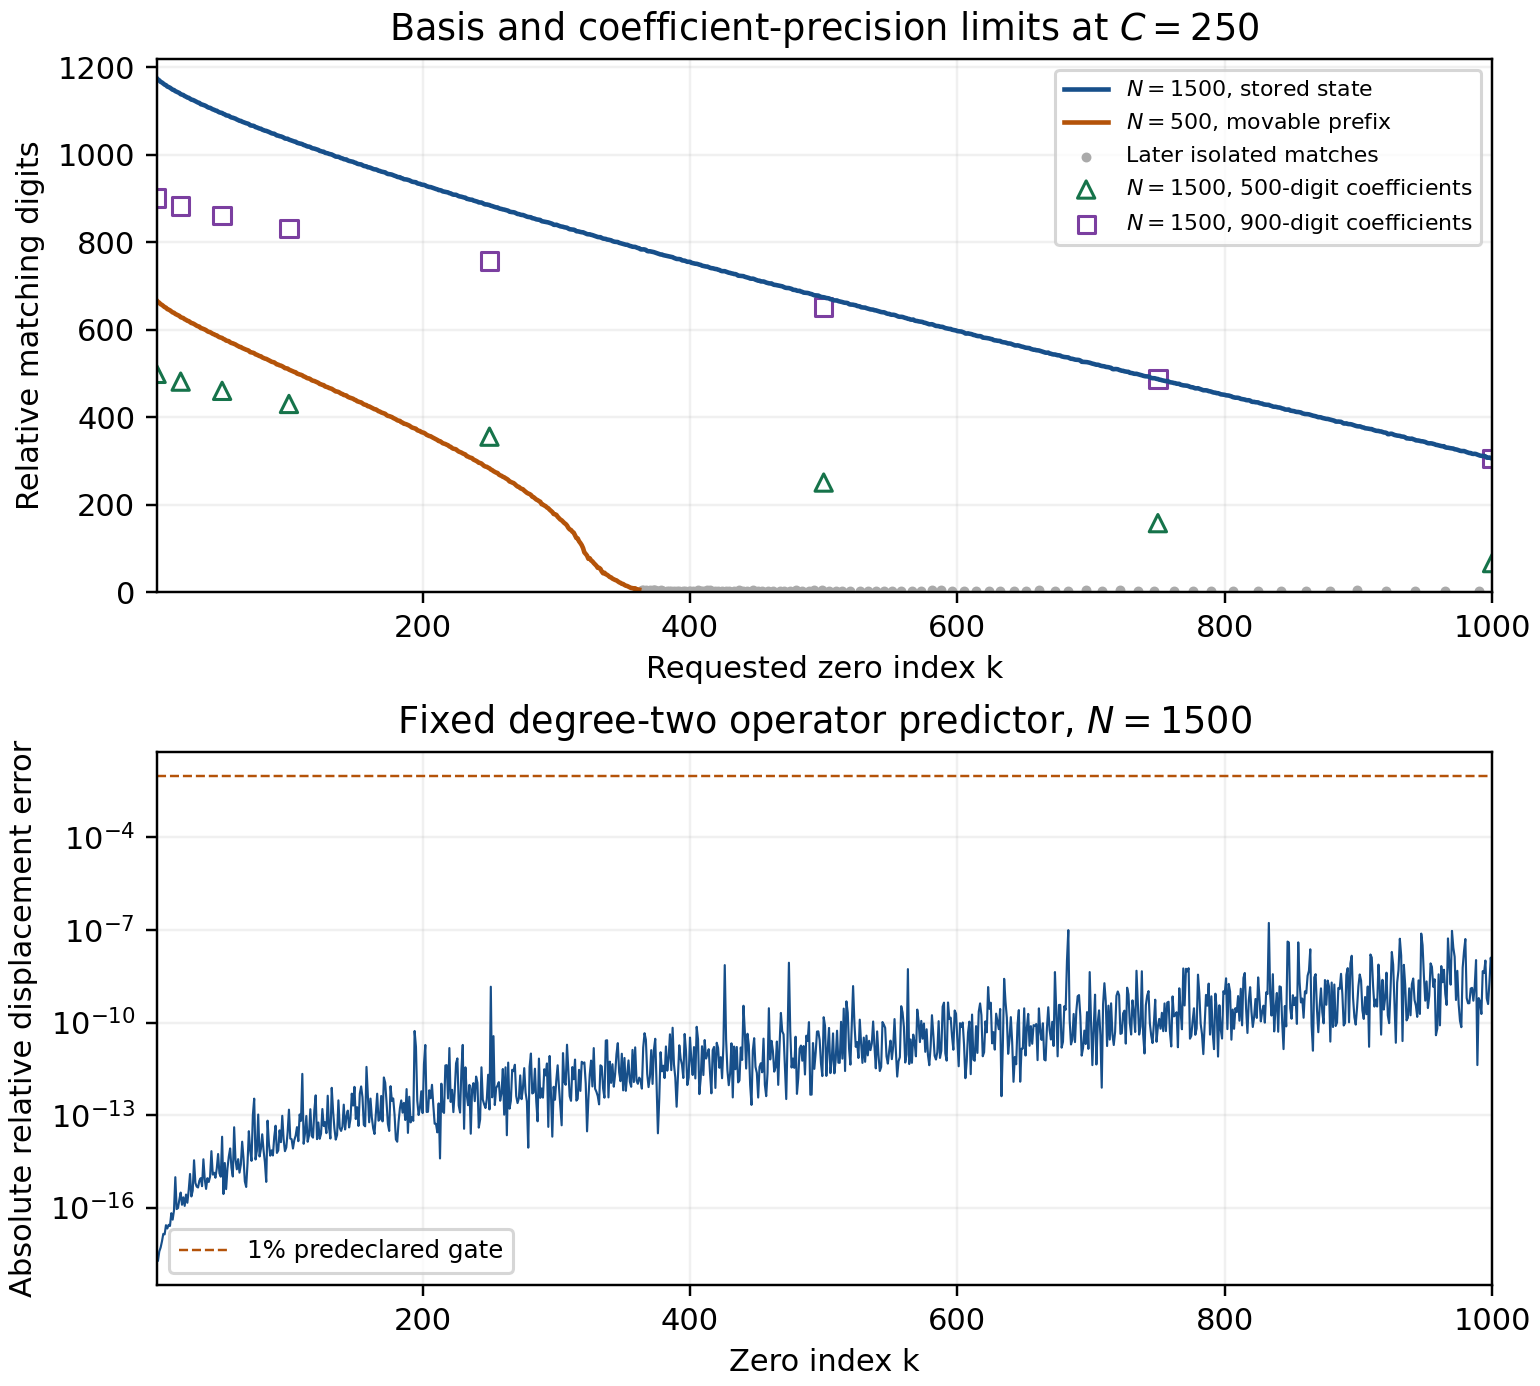
\includegraphics[width=.95\textwidth]{figures/indexed_campaign.png}
\caption{The same cutoff with different basis sizes and controlled
coefficient precision, followed by the fixed operator-predictor error on
the counted first-1000 prefix. Later isolated $N=500$ matches do not extend
its qualified movable prefix. All data concern retained point sources.}
\label{fig:thousand-zero-campaign}
\end{figure}

\paragraph{A derived refinement of the mode budget.}
Write the operator-predicted displacement as
$\widehat\delta_{N,k}=\varepsilon_N\mathcal T_{N,k}$, where
\[
 \mathcal T_{N,k}=
 \frac{\nu_{N,k}\sum_{i\in I_k}v_i Z_i/\varepsilon_N-S_{N,k}}
      {f_{N,k}^2},\qquad
 \mathcal R_{N,k}=\delta_{N,k}-\varepsilon_N\mathcal T_{N,k}.
\]
For associated roots at two basis sizes $N<M$, the exact finite increment is
\begin{align}\label{eq:energy-transfer-mode-split}
 \nu_{N,k}-\nu_{M,k}
  ={}&(\varepsilon_N-\varepsilon_M)\mathcal T_{M,k}\nonumber\\
    &+\varepsilon_N(\mathcal T_{N,k}-\mathcal T_{M,k})
      +(\mathcal R_{N,k}-\mathcal R_{M,k}).
\end{align}
This separates change in the eigenvalue with the parent transfer held
fixed, change in the indexed transfer, and the predictor remainder.
It is an algebraic identity, not a unique causal attribution: reversing
the order of the two changes produces another valid decomposition.
The three displayed terms sum to the finite increment and therefore do
not duplicate a fourth copy of the same mode error.

The transfer factor itself varies strongly with $N$ and $k$. At $C=250$,
write
\[
 \ell_k=\log_{10}|\mathcal T_{500,k}/\mathcal T_{1500,k}|.
\]
The computed values are
\[
\begin{array}{c|rrrrr}
k&1&19&100&250&350\\
\ell_k&0.05565&1.70202&17.73021&93.67247&269.55472
\end{array}
\]
In the parent-anchored split, the eigenvalue-change
term supplies $87.97\%$ of the increment at $k=1$, but only
$1.8612\cdot10^{-18}$ of it at $k=100$. A model that varies the
eigenvalue while holding this parent transfer factor fixed misses most
of the high-index change. These finite data rule out treating the
transfer factor as a function of $C,k$ alone over these two basis sizes.

If fixed-cutoff limits and branch correspondence are established, passing
$M\to\infty$ in~\eqref{eq:energy-transfer-mode-split} supplies an actual
mode decomposition. Relative upper bounds $B_E,B_T,B_R$ on its three
terms then give
\[
 D_{\mathrm{mode},k}\ge
 -\log_{10}(B_E+B_T+B_R)
 \ge\min\{D_E,D_T,D_R\}-\log_{10}3.
\]
This is a precise possible source of the additional indexed minimum:
the transfer term can limit accuracy even when the eigenvalue budget is
large. Its uniform CCM rate has not been derived. The finite comparison
uses independently assembled retained sources and supplies no bound on
the infinite remainder or assembly difference.

\paragraph{Remaining analytic task.}
The indexed minimum in~\eqref{eq:indexed-min-budget}, combined with a
valid branch gate, survives these tests. A closed law still requires
uniform CCM estimates for the primal residual, indexed dual tail,
root derivative, arithmetic cutoff contribution and numerical state
error. The exact count supplies a practical finite branch test, and the
operator moment rule supplies a precise correction target. Neither
replaces those missing estimates.
